\documentclass[border=3pt]{standalone}
% Preâmbulo compartilhado pelos diagramas TikZ da aula 7 de Navegação (Implementação do A*)
\usepackage[T1]{fontenc}
\usepackage[utf8]{inputenc}
\usepackage{lmodern}
\usepackage{amsmath}
\usepackage{xcolor}
\usepackage{tikz}
\usetikzlibrary{arrows.meta,angles,quotes,decorations.pathmorphing,decorations.pathreplacing,calc,
                positioning,shapes.geometric,shapes.misc,backgrounds,fit,
                math}

% Paleta (mesma dos SVGs originais)
\definecolor{dblue}{HTML}{2A5B8C}
\definecolor{dorange}{HTML}{B3541E}
\definecolor{dgreen}{HTML}{4A7C59}
\definecolor{dred}{HTML}{9C4B4B}
\definecolor{dcream}{HTML}{F4F1EA}
\definecolor{dshade}{HTML}{DDD7C9}

% Função gaussiana (não normalizada por padrão de escala visual)
\pgfmathdeclarefunction{gauss}{3}{%
  \pgfmathparse{1/(#3*sqrt(2*pi))*exp(-((#1-#2)^2)/(2*#3^2))}%
}

% Estilos comuns (prefixo d... para não colidir com chaves internas do pgf)
\tikzset{
  >={Stealth[length=2mm]},
  dguide/.style={gray!55, dashed, line width=0.4pt},
  daxis/.style={gray!60, line width=0.7pt, ->},
  dbody/.style={fill=black!3, draw=black!80, line width=1pt},
  dacc/.style={draw=dblue, line width=1pt},
  dlbl/.style={black!55, font=\small},
  dsub/.style={black!45, font=\footnotesize},
  dstate/.style={circle, draw=black!80, fill=dcream, line width=1pt,
                 minimum size=17mm, font=\large, inner sep=1pt},
  dobs/.style={circle, draw=black!80, fill=dshade, line width=1pt,
               minimum size=14mm, font=\large, inner sep=1pt},
  dbox/.style={rounded corners=2pt, draw=black!80, fill=dcream, line width=1pt,
               align=center, inner sep=6pt},
  dop/.style={circle, draw=black!80, fill=white, line width=1pt,
              minimum size=6mm, inner sep=0pt, font=\small},
  dtrans/.style={->, dblue, line width=1pt},
  dmeas/.style={->, dorange, line width=1pt},
  dcurve/.style={line width=1pt, dblue},
  dcurveb/.style={line width=1.4pt, dorange},
}

\begin{document}
\hyphenpenalty=10000 \exhyphenpenalty=10000 \tolerance=9999 \emergencystretch=3em
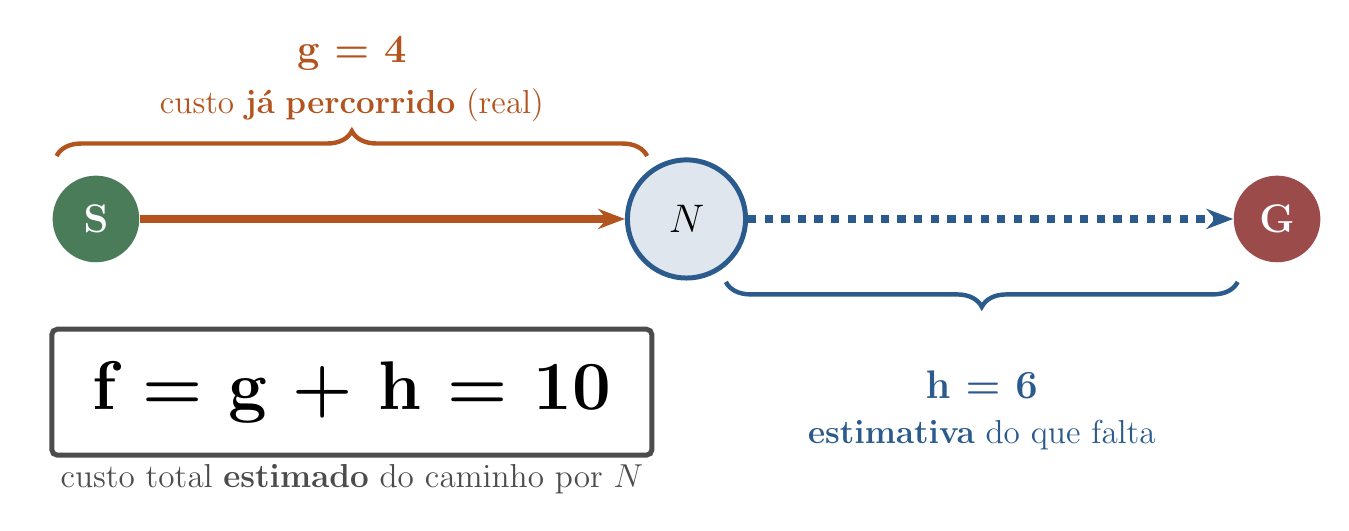
\begin{tikzpicture}[x=1cm,y=1cm]

\node[circle, fill=dgreen, text=white, font=\Large\bfseries, minimum size=1.1cm] (s) at (1.5,3.4) {S};
\node[circle, draw=dblue, fill=dblue!15, line width=1.8pt, font=\Large\bfseries, minimum size=1.5cm] (n) at (9.0,3.4) {$N$};
\node[circle, fill=dred, text=white, font=\Large\bfseries, minimum size=1.1cm] (g) at (16.5,3.4) {G};
\draw[dorange, line width=3pt, -{Stealth[length=3.4mm]}] (s) -- (n);
\draw[dblue, dashed, line width=3pt, -{Stealth[length=3.4mm]}] (n) -- (g);
\draw[decorate, decoration={brace, amplitude=9pt}, dorange, line width=1.6pt] (1.0,4.2) -- (8.5,4.2);
\node[font=\Large\bfseries, dorange, text width=8cm, align=center] at (4.75,5.5) {g = 4};
\node[font=\large, dorange, text width=8cm, align=center] at (4.75,4.85) {custo \textbf{já percorrido} (real)};
\draw[decorate, decoration={brace, amplitude=9pt, mirror}, dblue, line width=1.6pt] (9.5,2.6) -- (16.0,2.6);
\node[font=\Large\bfseries, dblue, text width=7cm, align=center] at (12.75,1.3) {h = 6};
\node[font=\large, dblue, text width=7cm, align=center] at (12.75,0.65) {\textbf{estimativa} do que falta};
\node[dbox, draw=black!70, fill=white, line width=1.8pt, text width=7.2cm, minimum height=1.6cm, font=\Huge\bfseries] at (4.75,1.2) {f = g + h = 10};
\node[font=\large, black!70] at (4.75,0.1) {custo total \textbf{estimado} do caminho por $N$};

\end{tikzpicture}
\end{document}
